\chapter{Clustering Agent Representations}
\label{chap:clustering_agent_representations}

\chapterepigraph{Our analysis shows that there are three kinds of people in the world: those who use $k$-means clustering with $k=3$, and two other types whose qualitative interpretation is unclear.}
{Randall Munroe, \textit{xkcd} no.~2731 (2023)~\parencite{munroe2023kmeans}}

\glsresetall

As discussed in the previous chapter, current explainability methods for \gls{rl} still lack intrinsic approaches capable of explaining the internal mechanisms of deep neural policies.
To the best of our knowledge, only \textcite{zahavy2017graying}, in their paper \citetitle{zahavy2017graying}, have proposed exploiting the \gls{ls} learned by neural policies in order to identify the concepts used by the agent.
Its main idea is to analyze the \glspl{lr} produced by the \gls{nn} and organize them into clusters that correspond to concepts.

While the core idea of this paper is closely aligned with our vision of explainability in \gls{rl}, this approach suffers from two important limitations.
First, the clusters are manually constructed.
Such a procedure heavily depends on the user's expertise and neither guarantees reproducibility or scales.
Second, no evaluation protocol is proposed to assess the quality of the obtained clusters.
Their relevance is essentially determined through visual inspection.

The \gls{car} method proposed in this chapter addresses these two limitations.
First, it automates concept discovery by relying on unsupervised clustering algorithms.
Second, it introduces an objective evaluation metric based on the stability of the extracted representations across independently trained policies.

This chapter is organized as follows:
\begin{itemize}
    \item Section~\ref{sec:clustering_agent_representations_representation_convergence_hypothesis} lays out the theoretical assumptions underlying the proposed \gls{car} method, which we term the \RepresentationConvergenceHypothesisName.
    \item Section~\ref{sec:clustering_agent_representations_latent_clustering_of_surrogate_policies} then details the \gls{car} method itself, covering both the extraction of \glspl{lr} using surrogate policies and the automatic detection of \glspl{cs} through clustering.
    \item Section~\ref{sec:clustering_agent_representations_evaluation_metrics} introduces the metrics we propose for evaluation.
    \item Section~\ref{sec:clustering_agent_representations_conclusion} situates \gls{car} within the broader landscape of \gls{me}.
\end{itemize}

\section{Representation Convergence Hypothesis}
\label{sec:clustering_agent_representations_representation_convergence_hypothesis}

The \gls{car} method relies on an assumption, referred to as the \RepresentationConvergenceHypothesisName.
This hypothesis follows the two assumptions established previously throughout this thesis.

The \MechanisticHypothesisName rejects the notion that deep \glspl{nn} constitute irreducible \enquote{black boxes}.
Adopting a mechanistic perspective, we consider that every process results from a sequence of causal computations.
Although these computations may be complex, they remain explainable through the analysis of the internal mechanisms.

The \ConceptHypothesisName states that \glspl{nn} achieve generalization by learning concepts.
During optimization, the network progressively organizes its \gls{ls} into representations that capture the information required to solve the task.

Following these two hypotheses, it becomes possible to explain a \gls{nn} by studying the organization of its \gls{ls}.
This family of approaches corresponds to \gls{me} (Definition~\ref{def:mechanistic_explainability}).
Since the \gls{car} method is grounded in these two hypotheses, it falls within this field of research.

More specifically, \gls{car} focuses on a specific aspect of \gls{me} known as universality.
Universality refers to the consistency with which a concept is recovered across different models trained on the same task \parencite{templeton2024scaling}.
In the literature, universality is mainly reported as an empirical observation, without an explanation of why it occurs.
In this thesis, we make it a central proposition for explaining \glspl{nn}.
If the same concepts emerge in every model trained on a task, these concepts characterize the task itself, and they can be used to explain the behavior of any of these models.

To provide an explanation for this phenomenon, we developed the \RepresentationConvergenceHypothesisName.
This hypothesis states that, when \glspl{nn} are trained to solve the same task, a set of concepts should systematically emerge because these concepts provide an effective way of representing the problem.
As a result, independently trained models should develop similar concepts in their learned representations.

\begin{hypothesis}{Representation Convergence Hypothesis}{convergence}
For a given task, independently trained \glspl{nn} tend to develop similar sets of concepts because these concepts provide an efficient representation for solving the task.
\end{hypothesis}

The \gls{car} method is designed to investigate the \RepresentationConvergenceHypothesisName by assessing whether it can consistently recover similar concepts across independently trained models.
The hypothesis therefore serves both as the foundation of the method and as the phenomenon it aims to investigate.

If \gls{car} consistently recovers the same set of concepts across different training runs, this set is more likely to reflect invariant properties of the task than model-specific artifacts.
Conversely, the absence of representation convergence would provide evidence against the hypothesis and would also question the validity of the \gls{car} approach.

It is important to clarify that this hypothesis does not imply convergence at the parameter level.
Independently trained models are expected to converge toward different sets of weights.
The proposed hypothesis concerns a abstract level of representation.
We assume that the conceptual organization induced by their \glspl{lr} converges toward an equivalent \gls{cs}, even though the numerical implementation of the networks differ.

The remainder of this chapter develops the methodology used to investigate this hypothesis.
\section{Latent Clustering of Surrogate Policies}
\label{sec:clustering_agent_representations_latent_clustering_of_surrogate_policies}

Following \textcite{zahavy2017graying}, we analyze the \gls{ls} through clustering techniques, placing our approach within the broader field of Deep Clustering.
This design choice is motivated by our rejection of the \SuperpositionHypothesisName and, more generally, of any view that assumes a linearly organized \gls{cs}, as discussed in Section~\ref{sec:latent_space_analysis_clustering}.

The \gls{car} methodology is composed of two main stages.
The first stage trains multiple independent \glspl{nn}, called surrogate policies, which implement the same decision policy.
The second stage clusters their \glspl{lr} in order to identify the underlying conceptual organization.
Once these two stages have been completed, the resulting clustering can be analyzed from two complementary perspectives.
First, the consistency of the resulting clusters across independent training runs can be assessed to determine whether the identified clusters are stable.
Second, the semantic content of the clusters can be examined to determine whether they correspond to meaningful concepts.
Figure~\ref{fig:illustration_method} provides a visual overview of the two stages, from the imitation of the initial policy to the clustering of the surrogate representations.

\begin{figure}[t]
    \centering
    \resizebox{\textwidth}{!}{
    \begin{tikzpicture}
        \node (observation) [minimum height=1.5cm, minimum width=2.5cm, align=center] at (0, 0) {\hl{Observation} \\ \large $o$};

        \node[draw, rectangle, text centered, minimum height=1cm, minimum width=2.5cm, align=center, rounded corners=0.2cm] (policy) at ($(observation) + (3cm, 1.35cm)$) {\scalebox{2}{$\InitialPolicy$}};

        \node[align=center] (policy_text) at ($(policy) + (0, 1cm)$) {Initial Policy};

        \node[draw, rectangle, text centered, minimum height=1cm, minimum width=2.5cm, align=center, rounded corners=0.2cm] (surrogate_policy) at ($(observation) + (3cm, -1.35cm)$) {\scalebox{2}{$\SurrogatePolicy{}$}};

        \node[align=center] (surrogate_policy_text) at ($(surrogate_policy) + (0, 1cm)$) {Surrogate Policy};

        \draw[->] (observation) |- (policy);
        \draw[->] (observation) |- (surrogate_policy);

        \def\B{4};
        \def\S{5};
        \def\Bs{1.0};
        \def\Ss{1.25};
        \def\xmax{\S+3.2*\Ss};

        \begin{axis}[
            name=policy_distribution,
            at={($(policy) + (5cm, 0cm)$)},
            anchor=center,
            every axis plot post/.append style={
                mark=none,domain={-0.05*(\xmax)}:{1.08*\xmax},samples=\numberOfSamplesToPlotCurve,smooth
            },
            xmin=0,
            xmax=\xmax,
            ymin=0,
            ymax={1.1*gauss(\B,\B,\Bs)},
            axis lines=middle,
            axis line style=thick,
            enlargelimits=upper, % extend the axes a bit to the right and top
            ticks=none,
            x=0.5cm,
            y=5cm,
            scale=0.7,
            xlabel={$\ActionSet$},
            xlabel style={at={(axis description cs:0.85,0.2)}, anchor=west},
            % ylabel={probability},
            ylabel style={at={(axis description cs:0,1.02)},anchor=south},
            title={action distribution},
            title style={at={(axis description cs:0.5,-0.15)},anchor=north},
        ]

        % PLOTS
        \addplot[name path=A,thick, mygreen] {gauss(x,\B,\Bs)} node[pos=0.5, above, xshift=-0.8cm, yshift=-0.2cm] {$\InitialPolicy\textcolor{black}{(o)}$};
        \end{axis}

        \begin{axis}[
            name=surrogate_policy_distribution,
            at={($(surrogate_policy) + (5cm, 0cm)$)},
            anchor=center,
            every axis plot post/.append style={
                mark=none,domain={-0.05*(\xmax)}:{1.08*\xmax},samples=\numberOfSamplesToPlotCurve,smooth
            },
            xmin=0,
            xmax=\xmax,
            ymin=0,
            ymax={1.1*gauss(\B,\B,\Bs)},
            axis lines=middle,
            axis line style=thick,
            enlargelimits=upper, % extend the axes a bit to the right and top
            ticks=none,
            x=0.5cm,
            y=5cm,
            scale=0.7,
            xlabel={$\ActionSet$},
            xlabel style={at={(axis description cs:0.85,0.2)}, anchor=west},
            % ylabel={probability},
            ylabel style={at={(axis description cs:0,1.02)},anchor=south},
            title={action distribution},
            title style={at={(axis description cs:0.5,-0.15)},anchor=north},
        ]

        % PLOTS
        \addplot[name path=B,thick,myred] {gauss(x,\S,\Ss)} node[pos=0.5, above, xshift=1.2cm, yshift=-0.3cm] {$\SurrogatePolicy{}\textcolor{black}{(o)}$};
        \end{axis}

        \draw[->] (policy) -- ($(policy_distribution.west) + (-0.2cm, 0)$);
        \draw[->] (surrogate_policy) -- ($(surrogate_policy_distribution.west) + (-0.2cm, 0)$);

        \begin{axis}[
            name=distribution_match,
            at={(13.5cm, 0cm)},
            anchor=center,
            every axis plot post/.append style={
                mark=none,domain={-0.05*(\xmax)}:{1.08*\xmax},samples=\numberOfSamplesToPlotCurve,smooth
            },
            xmin=0,
            xmax=\xmax,
            ymin=0,
            ymax={1.1*gauss(\B,\B,\Bs)},
            axis lines=middle,
            axis line style=thick,
            enlargelimits=upper, % extend the axes a bit to the right and top
            ticks=none,
            x=0.5cm,
            y=5cm,
            scale=0.8,
            xlabel={$\ActionSet$},
            xlabel style={at={(axis description cs:0.85,0.2)}, anchor=west},
            % ylabel={probability},
            ylabel style={at={(axis description cs:0,1.02)},anchor=south},
            title={\shortstack{difference between \\[0.08cm] distributions}},
            title style={at={(axis description cs:0.5,-0.15)},anchor=north},
        ]

        % PLOTS
        \addplot[name path=A,thick,mygreen] {gauss(x,\B,\Bs)} node[pos=0.5, above, xshift=-0.8cm, yshift=-0.2cm] {$\InitialPolicy\textcolor{black}{(o)}$};
        \addplot[name path=B,thick,myred] {gauss(x,\S,\Ss)} node[pos=0.5, above, xshift=1.2cm, yshift=-0.3cm] {$\SurrogatePolicy{}\textcolor{black}{(o)}$};

        \addplot[opacity=0.2] fill between[of=A and B, soft clip={domain=0:15}];
        \end{axis}

        \node[align=center] at ($(distribution_match.north) + (0, 1.25cm)$) {$\SurrogatePolicy{}$ is trained to be as close as \\ possible of $\InitialPolicy$ for all $o$ in order \\ to reproduce its behavior.};

        \draw[->] ($(policy_distribution.east) + (0.2cm, 0)$) -- ($(policy_distribution.east) + (0.5cm, 0)$) |- ($(distribution_match.west) + (-0.2cm, 0)$);
        \draw[->] ($(surrogate_policy_distribution.east) + (0.2cm, 0)$) -- ($(surrogate_policy_distribution.east) + (0.5cm, 0)$) |- ($(distribution_match.west) + (-0.2cm, 0)$);

        \begin{scope}[xshift=8cm, yshift=-5cm, scale=0.8, transform shape]
            \node[draw, minimum width=4cm, minimum height=4cm] (box_2) at (0, 0) {};

            \begin{scope}
                \clip (box_2.south west) rectangle (box_2.north east);

                \node[draw, dashed, minimum width=1.5cm, circle, minimum height=1.5cm] (circle_1) at (-1.25cm, -1.25cm) {};

                \node[draw, dashed, minimum width=1.5cm, circle, minimum height=1.5cm] (circle_2) at (0cm, 1.75cm) {};

                \node[draw, dashed, minimum width=1.5cm, circle, minimum height=1.5cm] (circle_3) at (1.75cm, 0cm) {};
            \end{scope}

            \foreach \x/\y in {
                -1.5/-0.75,
                -1.25/-1.5,
                -1/-1.75,
                -1.75/-1.25,
                -0.75/-1.25,
                -1/-1,
                0.5/1.5,
                -0.25/1.25,
                0.0/1.50,
                -0.5/1.5,
                0/1.25,
                1.5/-0.5,
                1.5/0.5,
                1.25/0.25,
                1.5/0,
                1.25/-0.25
            }
            {
                \node[] (p1) at (\x cm,\y cm) {\textcolor{myblue}{$\times$}};
            }
        \end{scope}
        \draw[->, dashed, preaction={draw=white,line width=6pt}] (surrogate_policy) |- ($(box_2.west) + (-0.2cm, 0)$);

        \node[draw, rectangle, text centered, align=center, dashed, fill=white, inner sep=1.5mm] at ($(surrogate_policy) - (0, 2.0cm)$) {Projection obtained through \\ the function $\SurrogateEncoder$, which is \\ a subcomponent of $\SurrogatePolicy{}$.};

        \node[align=center] at ($(box_2.east) + (2.75cm, 0)$) {Once $\SurrogatePolicy{}$ is trained,\\ observations are projected into $\LatentSet{}$,\\ clustered automatically,\\ and interpreted for semantics.};

        \node[align=center] at ($(box_2.south) + (0, -0.3cm)$) {\gls{ls} $\LatentSet{}$ of $\SurrogatePolicy{}$};
    \end{tikzpicture}
    }
    \caption{Illustration of the \methodName method.}
    \label{fig:illustration_method}
\end{figure}


This section is organized into three parts.
The first explains why multiple surrogate policies are used to study the stability of the representations.
The second describes how these policies are trained to match the initial policy as closely as possible.
The third presents how their \glspl{lr} are clustered to identify the \glspl{cs}.

\subsection{Multiple Surrogate Policies}

The \gls{car} method was developed to test the \RepresentationConvergenceHypothesisName.
This requires training several \glspl{nn} independently and comparing their \glspl{lr}.
Consistent similarities in the resulting \glspl{cs} would provide empirical support for this hypothesis.

In supervised learning, this protocol is straightforward since several models can be independently trained on the same target function.
\gls{rl} introduces an additional difficulty.
Because of stochastic exploration, independently trained agents are not guaranteed to converge toward the same policy.
Even if they achieve comparable performance, they may solve the task using different strategies.
This makes it difficult to determine whether differences in the \gls{ls} result from different representations of the same strategy or from differences in the learned strategies themselves.

To overcome this limitation, we consider an already trained initial policy.
This policy is then used as a target for imitation learning \parencite{pmlr-v15-ross11a}.
In this process, several surrogate \glspl{nn} are independently trained in a supervised manner to reproduce the behavior of the same agent.
This allows us to investigate whether \glspl{nn} that learn equivalent policies also develop similar conceptual organizations.

It is important to emphasize that the use of surrogate policies does not make \gls{car} a surrogate explainability method, as defined in Subsection~\ref{subsec:explainable_artificial_intelligence}.
The surrogate policies remain deep \glspl{nn}.
Their role is not to simplify the decision process but to provide multiple independent realizations of the same policy function, enabling the study of representation convergence.

\subsection{Training Surrogate Policies}

Throughout the remainder of this thesis, the initial policy we aim to explain is denoted as $\InitialPolicy$.
This initial policy is obtained without imposing any constraints on its origin.
It may result from classical or deep reinforcement learning \parencite{sutton2018reinforcement}, alpha-beta algorithm \parencite{knuth1975analysis}, or even from demonstrations provided by humans \parencite{pmlr-v9-ross10a}.
The crucial requirement is the availability of a dataset containing a sufficient number of projections from the observation space $\ObsSet$ to the action space $\ActionSet$ induced by $\InitialPolicy$ to train a \gls{nn}.

The replicated policies are referred to as surrogate policies.
To assess the stability of the learned representations, $n$ surrogate policies are trained independently, denoted by $\SurrogatePolicy{1}, \dots, \SurrogatePolicy{n}$.
All surrogate policies share the same architecture.
It consists of a \gls{nn} with two components, an encoder $\SurrogateEncoder$ and a decoder $\Decoder$, highlighted by the blue and black dashed rectangles, respectively, in Figure~\ref{fig:surrogate_policy_architecture}.
The encoder maps the observation $o$ to the embedding, and the decoder reconstructs the parameters of the action distribution from this embedding.
For a given surrogate policy $\SurrogatePolicy{i}$, parameterized by $\params_i$, its encoder and decoder are written $\SurrogateEncoder[i]$ and $\Decoder[i]$.

\begin{figure}[t]
    \centering
    \resizebox{\textwidth}{!}{
    \begin{tikzpicture}[x=3cm,y=1cm]
    \large
    \message{^^JDeep convolution neural network}
    \readlist\Nnod{4,5,6,5,3}
    \def\nstyle{1}
    \tikzset{
    node 1/.style={thick,circle,draw,minimum size=18,inner sep=0.5,outer sep=0.6},
    }

    \message{^^J  Layer}
    \foreachitem \N \in \Nnod{
        \def\lay{\Ncnt}
        \pgfmathsetmacro\prev{int(\Ncnt-1)}
        \message{\lay,}
        \foreach \i [evaluate={\y=\N/2-\i+0.5; \x=\lay; \n=\nstyle;}] in {1,...,\N}{ % loop over nodes
            \ifboolexpr{test {\ifnumcomp{\lay}{=}{3}}}
            {
                \node[node \n,outer sep=0.6] (N\lay-\i) at (\x,\y) {\textcolor{myblue}{$h^{(\lay)}_{\i}$}};
            }
            {
                \node[node \n,outer sep=0.6] (N\lay-\i) at (\x,\y) {};
            }

            \ifnum\lay>1
            \foreach \j in {1,...,\Nnod[\prev]}{ % loop over nodes in previous layer
                \draw[] (N\prev-\j) -- (N\lay-\i);
            }
            \fi
        }
    }

    \coordinate (policy_top_margin) at ($(N3-1) + (0, 1.3cm)$);
    \node[draw, rectangle, fit=(N1-1)(N3-6)(N5-1)(policy_top_margin), inner sep=0.25cm, dashed, rounded corners=0.3cm, color=myred] (policy) {};
      \node[] (policy_label) at ($(policy.north) + (0, 0.5cm)$) {\scalebox{2.5}{$\SurrogatePolicy{}$}};

    % Encoder box: encloses the layers up to and including the embedding
    \node[draw, dashed, rounded corners=0.15cm, color=myblue, fit=(N1-1)(N1-4)(N3-1)(N3-6), inner sep=0.15cm] (encoder_box) {};
    \node[align=center] (encoder_label) at ($(encoder_box.north) + (0, 0.5cm)$) {\scalebox{1.5}{$\SurrogateEncoder$}};

    % Decoder box: encloses the embedding and the layers up to the output
    \node[draw, dashed, rounded corners=0.15cm, color=black, fit=(N3-1)(N3-6)(N5-1), inner sep=0.15cm] (decoder_box) {};
    \node[align=center] (decoder_label) at ($(decoder_box.north) + (0, 0.5cm)$) {\scalebox{1.5}{$f_{dec}$}};

    % Observation
    \node[minimum height=1cm, minimum width=1cm] (observation_1) at ($(N1-1) + (-1.75cm, 0)$) {\scalebox{1.25}{$o_1$}};
    \node[minimum height=1cm, minimum width=1cm] (observation_2) at ($(N1-2) + (-1.75cm, 0)$) {\scalebox{1.25}{$o_2$}};
    \node[minimum height=1cm, minimum width=1cm] (observation_3) at ($(N1-3) + (-1.75cm, 0)$) {\scalebox{1.25}{$o_3$}};
    \node[minimum height=1cm, minimum width=1cm] (observation_4) at ($(N1-4) + (-1.75cm, 0)$) {\scalebox{1.25}{$o_4$}};

    \node[minimum height=1cm, minimum width=1cm, align=center] (observation_label) at ($(observation_1) + (0, 1.25cm)$) {\hl{Observation}};

    \draw[thick] (observation_1.north east) -- ($(observation_1.north east) + (-0.1cm, 0)$);
    \draw[thick] (observation_1.north east) -- (observation_4.south east);
    \draw[thick] (observation_4.south east) -- ($(observation_4.south east) + (-0.1cm, 0)$);

    \draw[thick] (observation_1.north west) -- ($(observation_1.north west) + (0.1cm, 0)$);
    \draw[thick] (observation_1.north west) -- (observation_4.south west);
    \draw[thick] (observation_4.south west) -- ($(observation_4.south west) + (0.1cm, 0)$);

    \draw[->] ($(observation_1.east) + (-0.15cm, 0)$) -- ($(N1-1.west) + (-0.0cm, 0)$);
    \draw[->] ($(observation_2.east) + (-0.15cm, 0)$) -- ($(N1-2.west) + (-0.0cm, 0)$);
    \draw[->] ($(observation_3.east) + (-0.15cm, 0)$) -- ($(N1-3.west) + (-0.0cm, 0)$);
    \draw[->] ($(observation_4.east) + (-0.15cm, 0)$) -- ($(N1-4.west) + (-0.0cm, 0)$);

    % Distribution
    \node[minimum height=1cm, minimum width=1cm] (distribution_1) at ($(N5-1) + (1.75cm, 0)$) {\scalebox{1.25}{$\ell_1$}};
    \node[minimum height=1cm, minimum width=1cm] (distribution_2) at ($(N5-2) + (1.75cm, 0)$) {\scalebox{1.25}{$\ell_2$}};
    \node[minimum height=1cm, minimum width=1cm] (distribution_3) at ($(N5-3) + (1.75cm, 0)$) {\scalebox{1.25}{$\ell_3$}};

    \draw[thick] (distribution_1.north east) -- ($(distribution_1.north east) + (-0.1cm, 0)$);
    \draw[thick] (distribution_1.north east) -- (distribution_3.south east);
    \draw[thick] (distribution_3.south east) -- ($(distribution_3.south east) + (-0.1cm, 0)$);

    \draw[thick] (distribution_1.north west) -- ($(distribution_1.north west) + (0.1cm, 0)$);
    \draw[thick] (distribution_1.north west) -- (distribution_3.south west);
    \draw[thick] (distribution_3.south west) -- ($(distribution_3.south west) + (0.1cm, 0)$);

    \draw[->] ($(N5-1.east) + (0.0cm, 0)$) -- ($(distribution_1.west) + (0.2cm, 0)$);
    \draw[->] ($(N5-2.east) + (0.0cm, 0)$) -- ($(distribution_2.west) + (0.2cm, 0)$);
    \draw[->] ($(N5-3.east) + (0.0cm, 0)$) -- ($(distribution_3.west) + (0.2cm, 0)$);

    \node[minimum height=1cm, minimum width=1cm, align=center] (distribution_label) at ($(distribution_1) + (0, 1.5cm)$) {Parameters \\ for the \\ \hl{Distribution}};

    % Embedding
    \node[align=center] (embedding_label) at ($(N3-6) + (0cm, -2cm)$) {\hl{Embedding}};

    \draw[thick, dashed, ->] ($(N3-6) + (0cm, -0.5cm)$) -- ($(embedding_label) + (0cm, 0.5cm)$);

    \node[] (embedding) at ($(embedding_label) + (0, -2cm)$) {
        $\begin{bmatrix}
            \textcolor{myblue}{h^{(3)}_{1}} \\
            \textcolor{myblue}{h^{(3)}_{2}} \\
            \textcolor{myblue}{h^{(3)}_{3}} \\
            \textcolor{myblue}{h^{(3)}_{4}} \\
            \textcolor{myblue}{h^{(3)}_{5}} \\
            \textcolor{myblue}{h^{(3)}_{6}}
        \end{bmatrix}$
    };

    \end{tikzpicture}
}
    \caption{Example of a surrogate policy architecture $\SurrogatePolicy{}$.}
    \label{fig:surrogate_policy_architecture}
\end{figure}


To train each surrogate policy $\SurrogatePolicy{i}$ to accurately replicate the action distribution, we define a loss function $\mathcal{L}$ optimized via gradient descent as introduced in Section~\ref{sec:deep_learning_learning}.
This loss, defined in Equation~\eqref{eq:car_loss}, is computed as the \gls{mse} between the parameters of the action distributions, obtained by applying the function $\logits$, which maps a distribution to its parameters (the logits).
In practice, this function $\logits$ does not need to be explicitly defined, as neural policies directly output the parameters of the action distribution.
Each surrogate policy $\SurrogatePolicy{i}$ is thus trained by solving:
\begin{align}
    \min_{\params_i} \sum_{o \in \ObsSet}
    \MSE\Big(
        \logits\big(\InitialPolicy\left(o\right)\big),
        \logits\big(\SurrogatePolicy{i}\left(o\right)\big)
    \Big).
    \label{eq:car_loss}
\end{align}

\subsection{Cluster Extraction}

Once the surrogate policies are trained, their encoders are used to generate a point cloud from a set of observations.
This point cloud provides a sample of the \gls{ls} to be analyzed.
The proposed \gls{car} method adopts the deep clustering approach introduced in Section~\ref{sec:latent_space_analysis_clustering}.
Under this approach, conceptually similar observations are expected to produce nearby \glspl{lr}.
A \gls{cs} can therefore be viewed as a region of the \gls{ls} containing related \glspl{lr}.
To identify these regions, a clustering algorithm is applied to the point cloud.

The clustering is performed independently for each surrogate policy.
For a surrogate policy $\SurrogatePolicy{i}$, applying its encoder $\SurrogateEncoder[i]$ to a subset of observations $\ObsData \subseteq \ObsSet$ yields the set of embeddings $\LatentSet{i}$.
A clustering function $\ClusteringFunction$ then partitions the point cloud $\LatentSet{i}$ into groups of nearby \glspl{lr}, assigning each observation a cluster label and yielding the partition $\mathcal{C}_{i}$.
The same observation set $\ObsData$ is used for every surrogate policy, so that the partitions $\mathcal{C}_{1}, \dots, \mathcal{C}_{n}$ are defined over the same observations and can be compared.
This comparison is the basis of the evaluation introduced in the following section.

Algorithm~\ref{alg:car} states the complete \gls{car} procedure, whose lines map directly onto the stages described above.
Lines~\ref{alg:car:dataset}--\ref{alg:car:loss} prepare the imitation of the initial policy.
They build the training dataset by pairing each observation with the parameters of the action distribution produced by $\InitialPolicy$, and define the \gls{mse} loss of Equation~\eqref{eq:car_loss}.
Lines~\ref{alg:car:train_loop}--\ref{alg:car:sgd} correspond to the first stage, in which each of the $n$ surrogate policies is initialized randomly and trained independently by stochastic gradient descent.
Lines~\ref{alg:car:cluster_loop}--\ref{alg:car:clust} correspond to the second stage.
The encoder of each surrogate policy embeds the shared observation set $\ObsData$ (Line~\ref{alg:car:embed}), and the resulting point cloud is partitioned by $\ClusteringFunction$ (Line~\ref{alg:car:clust}).
Finally, Line~\ref{alg:car:return} returns the surrogate policies together with their partitions, which are the inputs of the evaluation.

\begin{algorithm}[t]
\caption{\glsfmtlong{car} (\glsfmtshort{car})}
\label{alg:car}

\Input{
\\
Initial policy $\InitialPolicy$\\
Observation dataset $\ObsData$\\
Number of surrogate policies $n$\\
Surrogate policy architecture $\SurrogatePolicy{}$ (encoder $\SurrogateEncoder$, decoder $\Decoder$)\\
Learning rate $\eta$\\
Clustering function $\ClusteringFunction$
}

\Output{
\\
Trained surrogate policies $\SurrogatePolicy{1}, \dots, \SurrogatePolicy{n}$\\
Clusterings $\mathcal{C}_{1}, \dots, \mathcal{C}_{n}$
}

\AlgoRule

\tcp{Behavioral cloning dataset built from the target policy $\InitialPolicy$}
$\mathcal{D} \leftarrow \big\{ \big(o, \logits(\InitialPolicy(o))\big) \mid o \in \ObsData \big\}$\nllabel{alg:car:dataset}\;

\BlankLine
\tcp{MSE loss between action-distribution parameters, as defined in Equation~\eqref{eq:car_loss}}
$\mathcal{L} \leftarrow$ \gls{mse}\nllabel{alg:car:loss}\;

\BlankLine
\tcp{Independently train $n$ surrogate policies by behavioral cloning}
\For{$i = 1, \dots, n$\nllabel{alg:car:train_loop}}{
    Initialize $\params_i$ randomly\;

    \BlankLine
    \tcp{Behavioral cloning of $\InitialPolicy$ via SGD, see Algorithm~\ref{alg:stochastic_gradient_descent}}
    $\params_i \leftarrow$ \FnSGD{$\mathcal{D}, \SurrogatePolicy{}, \mathcal{L}, \eta, \params_i$}\nllabel{alg:car:sgd}\;
}

\BlankLine
\tcp{Cluster the latent representations of each surrogate policy}
\For{$i = 1, \dots, n$\nllabel{alg:car:cluster_loop}}{
    \tcp{Embeddings produced by the encoder of $\SurrogatePolicy{i}$}
    $\LatentSet{i} \leftarrow \big\{ \SurrogateEncoder[i](o) \mid o \in \ObsData \big\}$\nllabel{alg:car:embed}\;

    \BlankLine
    \tcp{Partition of the embedded observations into clusters}
    $\mathcal{C}_{i} \leftarrow \ClusteringFunction(\LatentSet{i})$\nllabel{alg:car:clust}\;
}

\BlankLine
\Return{\nllabel{alg:car:return}$\big(\SurrogatePolicy{1}, \dots, \SurrogatePolicy{n}\big), \big(\mathcal{C}_{1}, \dots, \mathcal{C}_{n}\big)$}

\end{algorithm}


Two choices govern this analysis without being part of the clustering algorithm itself.
The first is the choice of layer used to extract the representations.
Each hidden layer defines its own \gls{ls}, reflecting the information represented at that stage of the network.
\gls{car} can therefore be applied to the \glspl{lr} extracted from any layer.
This allows the conceptual organization of the policy to be examined at different levels of the network.

The second is the number of clusters.
\gls{car} does not assume that a task admits a single correct number of concepts.
This choice instead determines the granularity at which the conceptual organization is examined.
A small number reveals broad, strategic concepts, while a larger number reveals finer, tactical ones.
The influence of both choices is studied in Chapter~\ref{chap:experiments}.

Figure~\ref{fig:space_invaders_projection} shows the outcome of this procedure for a surrogate policy trained on \SpaceInvadersName, using five clusters.
The clusters are computed in the original high-dimensional \gls{ls}.
The point cloud is a two-dimensional projection used only for visualization.
Each cluster gathers observations that correspond to a distinct, interpretable stage of a game:
\begin{itemize}
    \item \textbf{Cluster 1:} The start of a game, with few or no invaders neutralized.
    \item \textbf{Cluster 2:} The right-hand group of invaders eliminated.
    \item \textbf{Cluster 3:} The pursuit of the bonus saucer.
    \item \textbf{Cluster 4:} The end of a game, with a few fast invaders close to the ground.
    \item \textbf{Cluster 5:} The middle of a game, with the invaders descending but already thinned out.
\end{itemize}

\NewDocumentCommand{\insertImageWithLine}{m m m m m}{
    \node[draw=#5, line width=6pt, inner sep=0] (#1) at (#2,#3) {
        \includegraphics[width=2.5cm]{#4}
    };
}

\definecolor{custom_blue}{HTML}{40568d}
\definecolor{custom_yellow}{HTML}{fee826}
\definecolor{custom_purple}{HTML}{440053}
\definecolor{custom_light_green}{HTML}{5eca61}
\definecolor{custom_dark_green}{HTML}{22928d}

\begin{figure}[t]
    \centering

    % --- Point cloud + cluster thumbnails, resized to \textwidth independently. ---
    % No longer tied to the legend's own scale factor, so it uses the full page
    % width on its own instead of being capped by the (wider) legend drawing.
    \resizebox{\textwidth}{!}{
        \begin{tikzpicture}
            \begin{pgfonlayer}{background}
                \node[anchor=south west,inner sep=0] (image) at (0,0) {
                    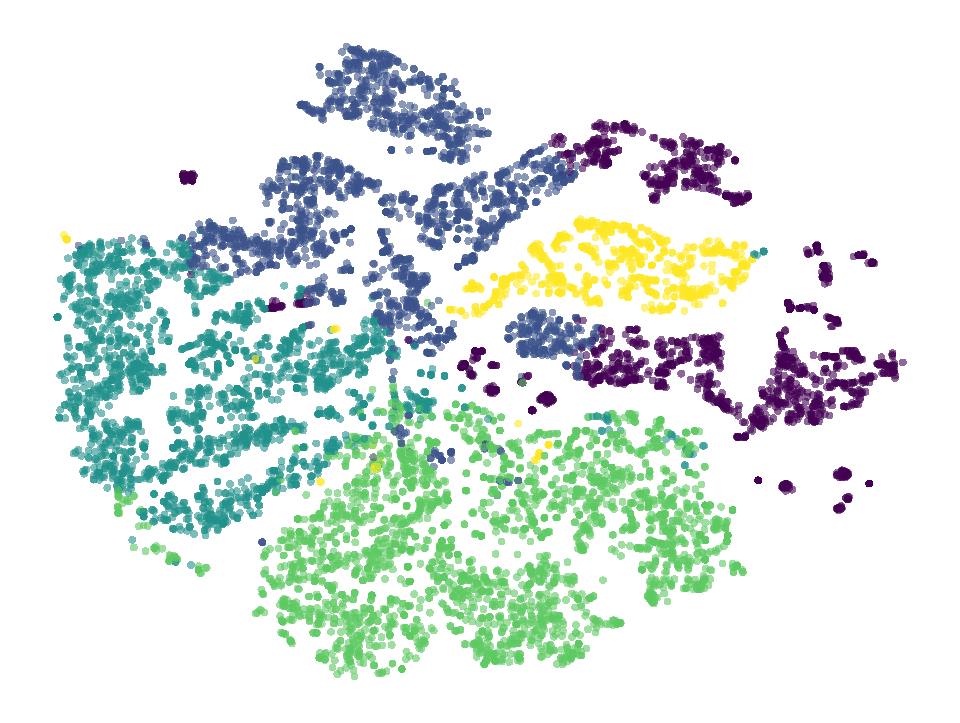
\includegraphics[]{figures/clustering_agent_representations/resources/projection_2d.pdf}
                };
            \end{pgfonlayer}

            \begin{scope}[x={(image.south east)},y={(image.north west)}]
                \node[circle, draw, inner sep=0.2cm, fill=white] (cluster_1) at (0.4,0.75) {\textbf{1}};
                \insertImageWithLine{image_1}{0.17}{0.85}{figures/clustering_agent_representations/pictures/space_invaders/5_clusters/early_game/image_1.png}{custom_blue}
                \insertImageWithLine{image_1}{0.35}{0.95}{figures/clustering_agent_representations/pictures/space_invaders/5_clusters/early_game/image_2.png}{custom_blue}

                \node[circle, draw, inner sep=0.2cm, fill=white] (cluster_2) at (0.65,0.63) {\textbf{2}};
                \insertImageWithLine{image_1}{0.57}{0.85}{figures/clustering_agent_representations/pictures/space_invaders/5_clusters/finish_right_group/image_1.png}{custom_yellow}
                \insertImageWithLine{image_1}{0.75}{0.85}{figures/clustering_agent_representations/pictures/space_invaders/5_clusters/finish_right_group/image_2.png}{custom_yellow}

                \node[circle, draw, inner sep=0.2cm, fill=white] (cluster_3) at (0.775,0.50) {\textbf{3}};
                \insertImageWithLine{image_1}{0.9}{0.55}{figures/clustering_agent_representations/pictures/space_invaders/5_clusters/catch_flying_saucer/image_1.png}{custom_purple}
                \insertImageWithLine{image_1}{0.85}{0.25}{figures/clustering_agent_representations/pictures/space_invaders/5_clusters/catch_flying_saucer/image_2.png}{custom_purple}

                \node[circle, draw, inner sep=0.2cm, fill=white] (cluster_4) at (0.525,0.25) {\textbf{4}};
                \insertImageWithLine{image_1}{0.65}{0.125}{figures/clustering_agent_representations/pictures/space_invaders/5_clusters/late_game/image_1.png}{custom_light_green}
                \insertImageWithLine{image_1}{0.40}{0.125}{figures/clustering_agent_representations/pictures/space_invaders/5_clusters/late_game/image_2.png}{custom_light_green}

                \node[circle, draw, inner sep=0.2cm, fill=white] (cluster_5) at (0.25,0.45) {\textbf{5}};
                \insertImageWithLine{image_1}{0.075}{0.50}{figures/clustering_agent_representations/pictures/space_invaders/5_clusters/mid_game/image_1.png}{custom_dark_green}
                \insertImageWithLine{image_1}{0.175}{0.20}{figures/clustering_agent_representations/pictures/space_invaders/5_clusters/mid_game/image_2.png}{custom_dark_green}
            \end{scope}
        \end{tikzpicture}
    }

    \vspace{0.2cm}

    % --- Legend, resized to \textwidth on its own. ---
    % Spacing between and within the two columns is untouched: same offsets, same
    % single-line entries, only the reference point moved from (image.south) to (0,0).
    % Since this legend was already the widest element in the original combined
    % figure, resizing it alone to \textwidth reproduces its original on-page size.
    \resizebox{\textwidth}{!}{
        \begin{tikzpicture}
            \node (element_1) at (-7cm, -1.5cm) {:};
            \node[anchor=west] (element_1_text) at ($(element_1) + (0.1cm, 0cm)$) {Projection of observations into the latent space.};
            \node[anchor=east] (element_1_symbol) at ($(element_1) + (-0.1cm, 0cm)$) {
                \tikz \fill[custom_blue] (0,0) circle (3pt);
                \tikz \fill[custom_yellow] (0,0) circle (3pt);
                \tikz \fill[custom_purple] (0,0) circle (3pt);
                \tikz \fill[custom_light_green] (0,0) circle (3pt);
                \tikz \fill[custom_dark_green] (0,0) circle (3pt);
                \hspace{0.02cm}
            };

            \node (element_2) at ($(element_1) + (0cm, -0.35cm)$) {:};
            \node[anchor=west] (element_2_text) at ($(element_2) + (0.1cm, 0cm)$) {Corresponding observations to the clusters.};
            \node[anchor=east] (element_2_symbol) at ($(element_2) + (-0.1cm, 0cm)$) {
                \tikz \draw[draw=custom_blue, fill=white, line width=0.5mm] (0,0) rectangle (2mm,2mm);
                \tikz \draw[draw=custom_yellow, fill=white, line width=0.5mm] (0,0) rectangle (2mm,2mm);
                \tikz \draw[draw=custom_purple, fill=white, line width=0.5mm] (0,0) rectangle (2mm,2mm);
                \tikz \draw[draw=custom_light_green, fill=white, line width=0.5mm] (0,0) rectangle (2mm,2mm);
                \tikz \draw[draw=custom_dark_green, fill=white, line width=0.5mm] (0,0) rectangle (2mm,2mm);
            };

            \node (element_3) at (3.4cm, -1cm) {:};
            \node[anchor=east] (element_3_symbol) at ($(element_3) + (-0.1cm, 0cm)$) {
                \textbf{Cluster 1} \tikz \fill[custom_blue] (0,0) circle (3pt);
            };
            \node[anchor=west] (element_3_text) at ($(element_3) + (0.1cm, 0cm)$) {Few or no invaders have been neutralized.};

            \node (element_4) at ($(element_3) + (0cm, -0.35cm)$) {:};
            \node[anchor=east] (element_4_symbol) at ($(element_4) + (-0.1cm, 0cm)$) {
                \textbf{Cluster 2} \tikz \fill[custom_yellow] (0,0) circle (3pt);
            };
            \node[anchor=west] (element_4_text) at ($(element_4) + (0.1cm, 0cm)$) {The invaders on the right side are eliminated.};

            \node (element_5) at ($(element_4) + (0cm, -0.35cm)$) {:};
            \node[anchor=east] (element_5_symbol) at ($(element_5) + (-0.1cm, 0cm)$) {
                \textbf{Cluster 3} \tikz \fill[custom_purple] (0,0) circle (3pt);
            };
            \node[anchor=west] (element_5_text) at ($(element_5) + (0.1cm, 0cm)$) {Try to catch the saucer that occasionally flies.};

            \node (element_6) at ($(element_5) + (0cm, -0.35cm)$) {:};
            \node[anchor=east] (element_6_symbol) at ($(element_6) + (-0.1cm, 0cm)$) {
                \textbf{Cluster 4} \tikz \fill[custom_light_green] (0,0) circle (3pt);
            };
            \node[anchor=west] (element_6_text) at ($(element_6) + (0.1cm, 0cm)$) {Few invaders remain, moving fast near ground.};

            \node (element_7) at ($(element_6) + (0cm, -0.35cm)$) {:};
            \node[anchor=east] (element_7_symbol) at ($(element_7) + (-0.1cm, 0cm)$) {
                \textbf{Cluster 5} \tikz \fill[custom_dark_green] (0,0) circle (3pt);
            };
            \node[anchor=west] (element_7_text) at ($(element_7) + (0.1cm, 0cm)$) {Invaders descend, but their numbers are reduced.};
        \end{tikzpicture}
    }

    \caption[Two-dimensional projection of a latent space for \SpaceInvadersName.]{Two-dimensional projection of the \glsfmtshort{ls} embeddings of a surrogate policy trained on \SpaceInvadersName, together with the \glsfmtshort{car} clusters and their corresponding observations.}
    \label{fig:space_invaders_projection}
\end{figure}


The position of an observation in the \gls{ls} thus reflects the stage of the environment it belongs to, suggesting a correspondence between the geometry of the \gls{ls} and the semantic properties of environment states.

This example illustrates what \gls{car} is expected to produce, but it relies on the visual inspection of a single surrogate policy, which is precisely the type of evidence whose limitations motivated this work.
Three aspects must therefore be evaluated before such an analysis can be trusted.
First, the surrogate policy must faithfully reproduce the initial policy so that its explanations remain relevant to the target policy.
Second, the recovered conceptual organization must be consistent across independently trained surrogate policies.
Finally, the clusters must capture genuine abstractions rather than simply reproducing structure already present in the observations or action distributions.

The following section introduces one evaluation metric for each of these aspects and details how it is computed.


\section{Evaluation Metrics}
\label{sec:clustering_agent_representations_evaluation_metrics}

To evaluate the effectiveness of \gls{car}, four evaluation metrics are introduced:

\begin{itemize}
    \item \textbf{\BehaviorReconstructionName} : it measures how well a surrogate policy faithfully reproduces the behavior of the initial policy by comparing their cumulative rewards.
    \item \textbf{\ClusteringUniversalityName} : it evaluates the stability of clusterings by measuring the similarity of clusters obtained from independently trained surrogate policies.
    \item \textbf{\AbstractionScoreName} : it quantifies the extent to which \gls{ls} clusters capture abstractions rather than directly reflecting the structure of observations, of the action distribution, or the network architecture prior to training.
    \item \textbf{\AdjustedClusteringUniversalityName}: it combines the two previous metrics to measure the agreement between surrogate policies beyond what can be explained by the baselines used in \AbstractionScoreName.
\end{itemize}

The remainder of this section details the motivation for each metric and describes how they are calculated.
In the first subsection, we develop the \BehaviorReconstructionName{}.
We then introduce the \gls{ari} measure, which serves as the foundation for the three other metrics introduced in the subsequent subsections, namely \ClusteringUniversalityName{}, \AbstractionScoreName{}, and \AdjustedClusteringUniversalityName{}.

\subsection{Behavior Reconstruction}

We introduce the \BehaviorReconstructionName metric to assess whether $\SurrogatePolicy{}$ faithfully reproduces the behavior of $\InitialPolicy$.
This metric compares the returns obtained by the initial policy $\InitialPolicy$ and the surrogate policies $\SurrogatePolicy{}$ over a set of evaluation episodes.
We use the definition of return introduced in Section~\ref{subsec:value_functions}, where $G_1$ denotes the discounted sum of rewards collected along a whole trajectory.
Here, the return is computed over complete episodes with $\gamma=1$, so $G_1$ corresponds to the total reward collected during the episode.
Each policy is evaluated over $M$ episodes.
We denote by $G^{(e)}_{\InitialPolicy}$ the return obtained by the initial policy in episode $e$, and by $G^{(e)}_{\SurrogatePolicy{j}}$ the return obtained by surrogate policy $\SurrogatePolicy{j}$ in episode $e$.
The \BehaviorReconstructionName{} is then defined as the mean return of the surrogate policies normalized by the mean return of the initial policy:

\begin{align}
    \BR = \frac{1}{n \sum_{e=1}^{M} G^{(e)}_{\InitialPolicy}} \sum_{j=1}^{n} \sum_{e=1}^{M} G^{(e)}_{\SurrogatePolicy{j}}
\end{align}

In imitation learning, it is unlikely to expect the surrogate policy $\SurrogatePolicy{}$ to outperform the initial policy $\InitialPolicy$ it aims to approximate through supervised learning \parencite{pmlr-v9-ross10a}.
Consequently this metric ranges in $[0,1]$.
Values approaching 1 indicate minimal loss in reproducing $\InitialPolicy$, while values close to 0 indicate poor reproduction.  

We deliberately adopt a reward-based definition rather than alternatives based on actions or action distributions (e.g., training loss, accuracy, KL divergence \parencite{shlens2014noteskullbackleiblerdivergencelikelihood}, or optimal transport \parencite{peyré2020computationaloptimaltransport}).
Since surrogate policies are trained in a supervised manner, they cannot develop strategies beyond those demonstrated by the initial policy.
This means that if the rewards achieved are comparable, the surrogate policy is effectively copying the initial policy's behavior.

\subsection{Adjusted Rand Index}
\label{subsec:adjusted_rand_index}

Within \gls{car}, concepts are assumed to correspond to clusters in the \gls{ls}.
Combined with the \RepresentationConvergenceHypothesisName, this suggests that independently trained surrogate policies should develop similar conceptual organizations.
Their \glspl{lr} should therefore produce similar clusterings when analyzed using the same clustering procedure.

When a particular observation is processed by the network, it is expected to activate the same concept regardless of the specific neural implementation of the policy.
If independently trained policies converge toward the same conceptual organization, a given observation should activate the same concept across all models.
As a consequence, observations grouped together within a cluster for one policy should also be grouped together for another independently trained policy.

In the clustering literature, the most used measures for comparing two partitions is the \gls{ari}~\parencite{hubert1985comparing}.
This measure quantifies the agreement between cluster assignments independently of the spatial organization of the clusters.
Both metrics introduced later in this chapter, \ClusteringUniversalityName{} and \AbstractionScoreName{}, rely on the \gls{ari}.
Since the \gls{ari} is a complex measure, we review its definition and discuss its main properties.

The \gls{ari} is derived from the \gls{ri}~\parencite{rand1971objective}, which measures the agreement between two partitions by considering every possible pair of points in the point cloud.
For each pair, four situations are possible:
\begin{itemize}
\item \textbf{Agreement:} The points belong to the same cluster in both partitions.
\item \textbf{Agreement:} The points belong to different clusters in both partitions.
\item \textbf{Disagreement:} The points belong to the same cluster in the first partition but to different clusters in the second.
\item \textbf{Disagreement:} The points belong to different clusters in the first partition but to the same cluster in the second.
\end{itemize}

The \gls{ri} measures the proportion of pairs for which the two partitions agree:
$$
\RI = \frac{\text{number of agreeing pairs}}{\text{total number of pairs}}.
$$

Although the \gls{ri} is intuitive, it suffers from an important limitation.
In most clustering problems, the majority of pairs of points belong to different clusters.
Consequently, even two completely independent partitions will agree on a large number of pairs, simply because both assign them to different clusters.
This effect becomes more pronounced as the number of points or clusters increases.

The \gls{ari} addresses this issue by accounting for the agreement that would be expected purely by chance.
It compares the observed agreement $\RI$ to the expected agreement under random partitions $\mathbb{E}[\RI]$.
The score is then normalized by the maximum agreement achievable beyond this random baseline, $\max(\RI) - \mathbb{E}[\RI]$.
As a result, an \gls{ari} of $0$ corresponds to the level of agreement expected from random clusterings, while an \gls{ari} of $1$ indicates perfect agreement between the two partitions:
\[
\ARI = \frac{\RI - \mathbb{E}[\RI]}{\max(\RI) - \mathbb{E}[\RI]}
\]

In practice, the \gls{ari} is computed directly from the cluster assignments of the two partitions.
Let clustering \(\mathcal{C}\) be composed of clusters \(\{C_i\}\) and clustering \(\mathcal{C}'\) of clusters \(\{C'_j\}\).
Let \(a_i = |C_i|\) denote the number of samples in cluster \(i\) of clustering \(\mathcal{C}\), and \(b_j = |C'_j|\) the number of samples in cluster \(j\) of clustering \(\mathcal{C}'\).
Furthermore, let \(n_{ij} = |C_i \cap C'_j|\) be the number of samples shared by cluster \(i\) of clustering \(\mathcal{C}\) and cluster \(j\) of clustering \(\mathcal{C}'\), and let \(N\) be the total number of samples.
With these definitions, the \gls{ari} can be computed as:

\[
\ARI =
\frac{
\sum_{i,j} \binom{n_{ij}}{2}
-
\left[
\sum_i \binom{a_i}{2}
\sum_j \binom{b_j}{2}
\right]
\big/ \binom{N}{2}
}{
\frac{1}{2}
\left[
\sum_i \binom{a_i}{2}
+
\sum_j \binom{b_j}{2}
\right]
-
\left[
\sum_i \binom{a_i}{2}
\sum_j \binom{b_j}{2}
\right]
\big/ \binom{N}{2}
}
\]

Because it is bounded by $1$, a value such as $0.5$ can be misleadingly interpreted as \enquote{halfway to a perfect match}.
This interpretation is incorrect because the \gls{ari} is normalized against the agreement expected from two random partitions.
As a result, values close to $1$ require the two clusterings to be nearly identical, while a value of $0.5$ already indicates substantial agreement~\parencite{amezquita2020orchestrating}.

\subsection{Clustering Universality}
\label{subsec:clustering_universality}

Having introduced the \gls{ari}, we can now define the \ClusteringUniversalityName metric.
While the \gls{ari} quantifies the similarity between two partitions, the objective of \gls{car} is to assess the consistency of conceptual organizations across an entire set of independently trained surrogate policies.

To this end, the same set of observations is projected into the \gls{ls} of each surrogate policy and clustered.
Under the \RepresentationConvergenceHypothesisName, these independently obtained partitions are expected to be similar.
\ClusteringUniversalityName{} quantifies this by computing the mean pairwise \gls{ari}:

\begin{align}
    \CU
    =
    \frac{1}{\binom{n}{2}}
    \sum_{i=2}^{n}
    \sum_{j=1}^{i-1}
    \ARI(\mathcal{C}_{i}, \mathcal{C}_{j}).
\end{align}

This metric takes values in $[-1, 1]$.
A value close to $1$ indicates that surrogate policies produce highly similar partitions, suggesting that the clusters reflect intrinsic properties of the policy.
Conversely, a value near $0$ implies that the similarity between partitions is no better than that of two randomly generated clusterings, meaning that the clustering fails to capture any meaningful structure in the policy.
A negative value, on the other hand, signals that the agreement between partitions is worse than what would be expected by chance, indicating a systematic disagreement between the clusterings.

Figure~\ref{fig:clustering_universality_illustration} illustrates \ClusteringUniversalityName{} in the ideal case.
It shows three \glspl{ls} obtained by projecting the same seven observations, labeled 1 to 7, through three independently trained surrogate policies.
Although the embeddings occupy different positions, the clusters group exactly the same elements in all three cases.
The partitioning is therefore identical, resulting in an \gls{ari} of $1$.

% --- Macro pour une surrogate policy + son ensemble ---
\newcommand{\surrogatepolicy}[7]{%
    % #1 : xshift
    % #2 : index (1,2,3,…)
    % #3 : liste des coordonnées X des points
    % #4 : liste des coordonnées Y des points
    % #5 : liste des coordonnées X des circlepattern
    % #6 : liste des coordonnées Y des circlepattern
    % #7 : liste des diamètres des circlepattern
    \node[policybox] (policy#2) at (#1,0)
        {\scalebox{2}{$\SurrogatePolicy{#2}$}};

    \begin{scope}[xshift=#1, yshift=-4cm, scale=0.8, transform shape]
        \node[pointset] (box#2) at (0,0) {};
        \begin{scope}
            \clip (box#2.south west) rectangle (box#2.north east);
            % Circlepattern avec diamètres spécifiques
            \foreach \cx/\cy [count=\i] in {#5} {
                \pgfmathsetmacro{\currentcy}{{#6}[\i-1]}
                \pgfmathsetmacro{\diameter}{{#7}[\i-1]}
                \node[draw, dashed, circle, minimum size=\diameter] at (\cx cm, \currentcy cm) {};
            }
        \end{scope}

        % Points avec E_i dans un cercle bleu
        \foreach \x/\y [count=\i] in {#3} {
            \pgfmathsetmacro{\currenty}{{#4}[\i-1]}
            \node[draw=myblue, circle, inner sep=2pt, fill=white] at (\x cm, \currenty cm) {\scalebox{0.8}{\textcolor{myblue}{\small $\i$}}};
        }
    \end{scope}
    \draw[->, dashed, preaction={draw=white,line width=6pt}] (policy#2) -- ($(box#2.north)+(0,0)$);
}

\begin{figure}[t]
    \centering
    \resizebox{\textwidth}{!}{
    \begin{tikzpicture}[
        policybox/.style={
            draw, rectangle, text centered,
            minimum height=1cm, minimum width=2.5cm,
            align=center, rounded corners=0.2cm
        },
        pointset/.style={
            draw, minimum width=4cm, minimum height=4cm
        },
        circlepattern/.style={
            draw, dashed, circle, minimum width=1.5cm, minimum height=1.5cm
        }
    ]

    % --- Utilisation de la macro pour les trois policies ---
    \surrogatepolicy
    {-6cm}
    {1}
    {-1.5, -1.25, -1, 1.35, 1.0, -0.25, 0.25}
    {-0.75, -1.5, -1, 0.5, 0.0, 1.6, 1.6}
    {-1.25, 1.2, 0}
    {-1.1, 0.2, 1.75}
    {1.5cm, 1.25cm, 1.25cm}

    \surrogatepolicy
    {0cm}
    {2}
    {1, 1.3, 1.5, 0.1, 0.25, 0.45, 1.2}
    {1.5, 1, 1.5, 0.75, 0.2, -1.5, -1}
    {1.25, 0.1, 0.8}
    {1.3, 0.4, -1.2}
    {1.3cm, 1.2cm, 1.6cm}

    \surrogatepolicy
    {6cm}
    {3}
    {0.0, -0.5, 0.25, -1, -1.5, 1.6, 1.2}
    {0.0, 0.5, 0.5, -1.5, -1, 1.2, 1.6}
    {-1.25, -0.15, 1.5}
    {-1.25, 0.3, 1.5}
    {1.3cm, 1.5cm, 1.3cm}

    % --- Acolade et équation en dessous ---
    \draw[
        line width=1pt,  % Épaisseur du trait
        decorate,
        decoration={
            brace,
            amplitude=20pt,  % Hauteur de l'acolade
            mirror,          % Acolade sous la ligne
            raise=10pt       % Décalage vertical
        }
    ]
        (-8.5, -5.5) -- (8.5, -5.5);

    \node[below=0.75cm] at (0, -6) {
        \scalebox{1.5}{$\displaystyle
        \CU = 1
        $}
    };

    \end{tikzpicture}
    }
    \caption[Illustration of \glsfmtshort{cu} in the ideal case.]{Illustration of \glsfmtshort{cu} in the ideal case where projections of the same observations are grouped within the same clusters across all surrogate policies.}
    \label{fig:clustering_universality_illustration}
\end{figure}


\subsection{Abstraction Score}
\label{subsec:abstraction_score}

If \ClusteringUniversalityName is high, it becomes important to determine what underlies this stability.
Two possibilities arise:
\begin{enumerate}[label=(\roman*), ref=(\roman*)]
\item \label{i} the \gls{ls} provides no abstraction, as defined in Definition~\ref{def:abstraction}, because it either reproduces the observation space or action distribution, or reflects a structure already present in the network architecture before training;
\item \label{ii} the \gls{ls} captures similarities in decision-making, resulting in behaviorally meaningful clusters.
\end{enumerate}

To distinguish among these cases, we introduce the \AbstractionScoreName.
This metric contextualizes latent clusterings by examining how their patterns align with three reference baselines: the raw observations, the action distribution of the initial policy, and an untrained network of the same architecture.

We consider $\BaselineClustering{obs}$, the clustering of the observations $\ObsData$, and $\BaselineClustering{act}$, the clustering of the action distribution of the initial policy.
Concretely, $\BaselineClustering{act}$ is computed on the parameters of this distribution (the logits, before the softmax) produced by the initial policy for the same observations, which are precisely the quantities the surrogate policies are trained to reproduce.
We cluster these continuous parameters rather than the sampled discrete action, since a discrete action takes only a few distinct values, which would limit the number of clusters that can be distinguished.
Both clusterings use the same algorithm, distance metric, and hyperparameters as those used for $\mathcal{C}_{i}$ in the \gls{ls}.
This ensures that the three clusterings are obtained under the same conditions.

The third baseline addresses the case where the \gls{ls} merely reflects an inductive bias of the network architecture rather than something learned.
To this end, we introduce $U$ untrained networks sharing the same architecture as the surrogate policies, but with randomly initialized, never-updated weights.
Each of these $U$ untrained networks is used to project the same observations into its own latent space, which is then clustered in the same way, yielding partitions $\BaselineClustering[1]{untr}, \dots, \BaselineClustering[U]{untr}$.
This baseline isolates what the architecture already imposes on the representation before any learning takes place, so that a high similarity between $\mathcal{C}_i$ and this baseline indicates that the corresponding structure cannot be attributed to training.

For each latent clustering $\mathcal{C}_{i}$, we define its similarity to these three baselines using the \gls{ari}:

\begin{align*}
\Similarity{obs}{i} &= \ARI(\mathcal{C}_{i}, \BaselineClustering{obs}) \\
\Similarity{act}{i} &= \ARI(\mathcal{C}_{i}, \BaselineClustering{act}) \\
\Similarity{untr}{i} &= \frac{1}{U} \sum_{u=1}^{U} \ARI(\mathcal{C}_{i}, \BaselineClustering[u]{untr})
\end{align*}

The \AbstractionScoreName is subsequently calculated as one minus the average of the maximum absolute similarity values across these three reference baselines:

\begin{align}
\scalebox{0.9}{%
$\AS = 1 - \frac{1}{n} \sum_{i=1}^{n} \max \left( \left|\Similarity{obs}{i}\right|, \left|\Similarity{act}{i}\right|, \left|\Similarity{untr}{i}\right| \right)$%
}
\end{align}

The \AbstractionScoreName ranges from $[0, 1]$.
A score around $0$ means that the latent clusters are strongly aligned with the observation space, the action distribution, or the untrained network, reflecting no abstraction, case~\ref{i}.
A score close to $1$ indicates that the latent clusters are independent of the observation space, the action distribution, and the network's initialization, capturing abstractions that meaningfully reflect the agent's behavior, case~\ref{ii}.

\subsection{Adjusted Clustering Universality}
\label{subsec:adjusted_clustering_universality}

As discussed above, \ClusteringUniversalityName alone does not indicate whether the recovered structure is meaningful.
We therefore introduce the \AdjustedClusteringUniversalityName, which measures how much of the agreement between the different surrogate policies remains after accounting for the three trivial baselines.

\begin{align}
\scalebox{1}{%
$\ACU
=
\CU
-
\frac{1}{n}\sum_{i=1}^{n}
\max\left(
\left|\Similarity{obs}{i}\right|,
\left|\Similarity{act}{i}\right|,
\left|\Similarity{untr}{i}\right|
\right)$%
}
\end{align}

This metric ranges in $[-1, 1]$.
A value close to $1$ indicates that surrogate policies converge toward a partition that is both highly reproducible across seeds and clearly not explained by the observation space, the action distribution, or the network's initialization, providing the strongest evidence for \RepresentationConvergenceHypothesisName.
A value close to $0$, or negative, indicates that whatever agreement exists between independently trained surrogate policies is largely trivial: the surrogate policies converge, but toward a partition that could just as easily emerge from raw pixel similarity, from the action distribution of the initial policy, or from an untrained network sharing the same architecture.

\section{Conclusion}
\label{sec:clustering_agent_representations_conclusion}

The \gls{car} method was developed to investigate how concepts are organized within the representations of \gls{rl} policies.
It is based on three hypotheses introduced throughout this thesis, the \MechanisticHypothesisName, the \ConceptHypothesisName, and the \RepresentationConvergenceHypothesisName.

\gls{car} translates these assumptions into an empirical analysis.
Multiple surrogate policies are trained independently to reproduce the same policy.
Their \glspl{lr} are then clustered and compared to assess whether similar conceptual structures emerge across policies.
The \ClusteringUniversalityName and \AbstractionScoreName provide quantitative measures for evaluating the consistency and abstraction of the resulting clusters.

This makes \gls{car} a general procedure for analyzing agent representations.
The analysis and evaluation metrics are fully automated and require no manual intervention or environment-specific adjustments.
The method can therefore be applied to a wide range of \gls{rl} settings and provides a basis for systematically studying the internal representations of neural policies.

The next chapter applies \gls{car} to several environments to evaluate its ability to identify meaningful conceptual structures.


